% Copyright 2004 by Till Tantau <tantau@users.sourceforge.net>.
%
% In principle, this file can be redistributed and/or modified under
% the terms of the GNU Public License, version 2.
%
% However, this file is supposed to be a template to be modified
% for your own needs. For this reason, if you use this file as a
% template and not specifically distribute it as part of a another
% package/program, I grant the extra permission to freely copy and
% modify this file as you see fit and even to delete this copyright
% notice. 

\documentclass{beamer}
\usepackage[utf8]{inputenc}
%\usepackage{wrapfig}
\usepackage{array}
\usepackage{hyperref}
\usepackage{pdfpages}
%\usepackage{cellspace}
% There are many different themes available for Beamer. A comprehensive
% list with examples is given here:
% http://deic.uab.es/~iblanes/beamer_gallery/index_by_theme.html
% You can uncomment the themes below if you would like to use a different
% one:
%\usetheme{AnnArbor}
%\usetheme{Antibes}
%\usetheme{Bergen}
%\usetheme{Berkeley}
%\usetheme{Berlin}
%\usetheme{Boadilla}
%\usetheme{boxes}
%\usetheme{CambridgeUS}
%\usetheme{Copenhagen}
%\usetheme{Darmstadt}
%\usetheme{default}
%\usetheme{Frankfurt}
%\usetheme{Goettingen}
%\usetheme{Hannover}% attend j'essaie juste pour voir si je peut le logo  du noyau de linux au debut ok , j'ai deja compris msium
%\usetheme{Ilmenau}
%\usetheme{JuanLesPins}
%\usetheme{Luebeck}
%\usetheme{Madrid}
%\usetheme{Malmoe}
%\usetheme{Marburg}
%\usetheme{Montpellier}
%\usetheme{PaloAlto}
%\usetheme{Pittsburgh}
%\usetheme{Rochester}
\usetheme{Singapore}
%\usetheme{Szeged}
%\usetheme{Warsaw}

%\title{Distribution de Linux/(GNU/LINUX)}



% A subtitle is optional and this may be deleted
%\subtitle{GNU/Linux}

%\author{BEYA NTUMBA Joel   \and MAMADOU DJOULDE Barry}
 %- Give the names in the same order as the appear in the paper.
 %- Use the \inst{?} command only if the authors have different
   %affiliation.

%\institute[Universities of Somewhere and Elsewhere] % (optional, but mostly needed)
%{
  %\inst{1}%
 % Université de Montpellier - Faculté des Sciences
  
%} 

 % \and
  %\inst{2}%
  %Department of Theoretical Philosophy\\
  %University of Elsewhere}
% - Use the \inst command only if there are several affiliations.
% - Keep it simple, no one is interested in your street address.

%\date{Conference Name, 2013}
% - Either use conference name or its abbreviation.
% - Not really informative to the audience, more for people (including
%   yourself) who are reading the slides online

%\subject{Theoretical Computer Science}
% This is only inserted into the PDF information catalog. Can be left
% out. 

% If you have a file called "university-logo-filename.xxx", where xxx
% is a graphic format that can be processed by latex or pdflatex,
% resp., then you can add a logo as follows:

% \pgfdeclareimage[height=0.5cm]{university-logo}{university-logo-filename}
% \logo{\pgfuseimage{university-logo}}

% Delete this, if you do not want the table of contents to pop up at
% the beginning of each subsection:
%\AtBeginSubsection[]
%{
  %\begin{frame}<beamer>{Introduction}
    %ù\tableofcontents[currentsection,currentsubsection]
%\end{frame}
%}

% Let's get started
\begin{document}

%% CREATED BY DAVID FRISK, 2016

% COVER PAGE
\begin{titlepage}
\newgeometry{top=3cm, bottom=3cm,
			left=2.25 cm, right=2.25cm}	% Temporarily change margins		
			
% Cover page background 
\AddToShipoutPicture*{\backgroundpic{-4}{56.7}{figure/auxiliary/begin.pdf}}
\addtolength{\voffset}{2cm}

% Cover picture (replace with your own or delete)		
\begin{figure}[H]
\centering
\vspace{2cm}	% Adjust vertical spacing here
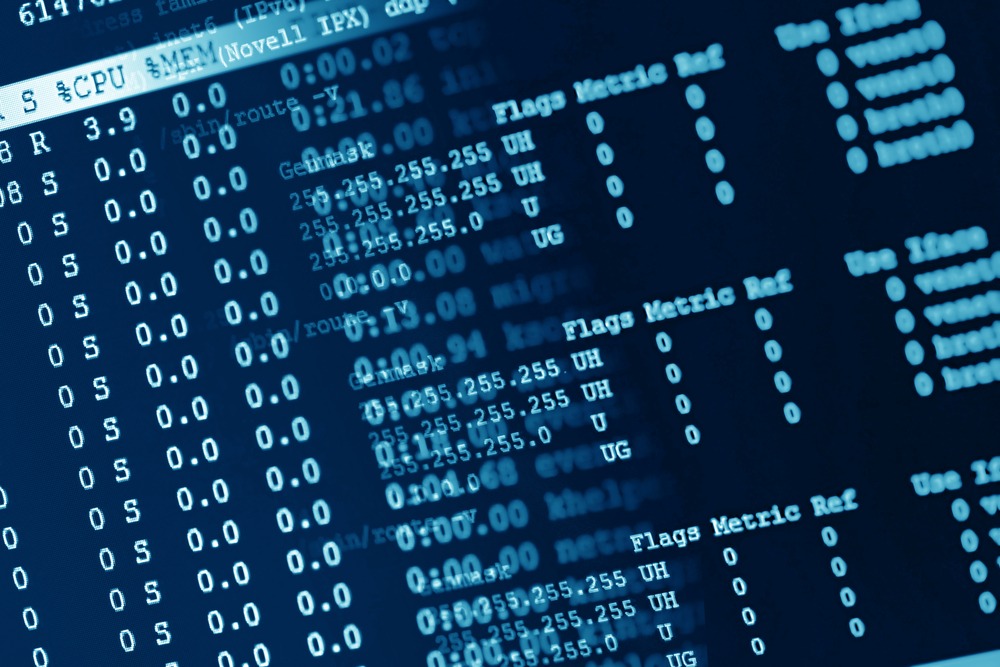
\includegraphics[width=0.9\linewidth]{figure/int.jpg}
\end{figure}

\textbf{{\Huge 	INTERPRÉTEUR DE COMMANDES }}	\\[0.2cm] 
%Licence Informatique \setlength{\parskip}{1cm}

\large{
\begin{itemize}[label=$\square$]
\item JONATHAN TWAMBA SAIBA
\item IBRAHIMA TOUNKARA
\item JOEL BEYA NTUMBA
\end{itemize}}

\begin{itemize}
\item Encadrant : \large{MICHEL LECLÈRE}
\end{itemize}

% Cover text
%\mbox{}
\vfill
%\renewcommand{\familydefault}{\sfdefault} \normalfont % Set cover page font
Département Informatique \\
\textsc{Université de Montpellier} \\
Montpellier, France 2017

%\renewcommand{\familydefault}{\rmdefault} \normalfont % Reset standard font
\end{titlepage}

\begin{frame}
\begin{center}

\includegraphics[scale=0.25]{begine.png}
\end{center}
\end{frame}

%\begin{frame}
%  \titlepage
%\end{frame}

\begin{frame}{Sommaire}
  \tableofcontents
  % You might wish to add the option [pausesections]
\end{frame}

\begin{frame}{Avant-propos}
 \begin{block}
\raggedright Linux a le vent en poupe depuis un certain nombre d'années et sa popularité croissante encourage de plus en plus à faire le grand saut. Cette aventure commence par le choix d'une distribution, décision importante car chacune a ses particularités. Autant s'épargner de futurs efforts inutiles de migration !
\end{block}  
\end{frame}
% Section and subsections will appear in the presentation overview
% and table of contents.
\section{Introduction}
\begin{frame}{Introduction}
\begin{block}
\raggedright 
Pour pouvoir parler de distributions LINUX, il faut savoir ce qu'est le noyau linux, système d'exploitation et l'ensemble du projet GNU. Mais on ne s'interessera pas à ceux là, considérant qu'une telle procédure dépasse largement le cadre de cette présentation. Néanmoins on pourra les énoncer dans l'historique.  
\end{block}
\end{frame}

\begin{frame}{}
\begin{block}{Définition}
%\begin{block}{definition}
%\end{block}
\raggedright 
Une distribution Linux est un système d'exploitation complet incluant un noyau Linux, un programme d'installation, et surtout des applications et utilitaires transformant l'ordinateur en outil réellement exploitable.
\end{block}
\end{frame}

\section{Historique}
\begin{frame}{}

%begin{block}{definition}
%\end{block}
 \begin{block}{GNU/Linux}
 GNU/Linux est un système d'exploitation associant des éléments essentiels du projet GNU et le noyau Linux. \\ 
 
\raggedright \centering
\includegraphics[height=3cm, width=6cm]{popo.png}
\end{block}
\end{frame}
%\end{frame}

\begin{frame}{}
\begin{block}{Projet GNU}
\raggedright Le projet GNU est un projet informatique dont les premiers développements ont été réalisés en janvier 1984 par Richard Stallman pour développer le système d'exploitation complet compatible unix, le GNU.\\ 
\centering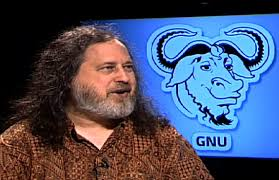
\includegraphics[height=4.5cm, width=7cm]{rich_gnu.jpg}
\end{block}
\end{frame}

\begin{frame}{Linux}
\begin{block}{}
Linux est un noyau de système d'exploitation de type UNIX crée par Linus Torvalds en 1991. Il gère les ressources de l’ordinateur et permet aux différents composants — matériels et logiciels — de communiquer entre eux. . Et donc un assemblage de distribution autour du dit noyau permet de fournir un système clé en main.\\ 
\centering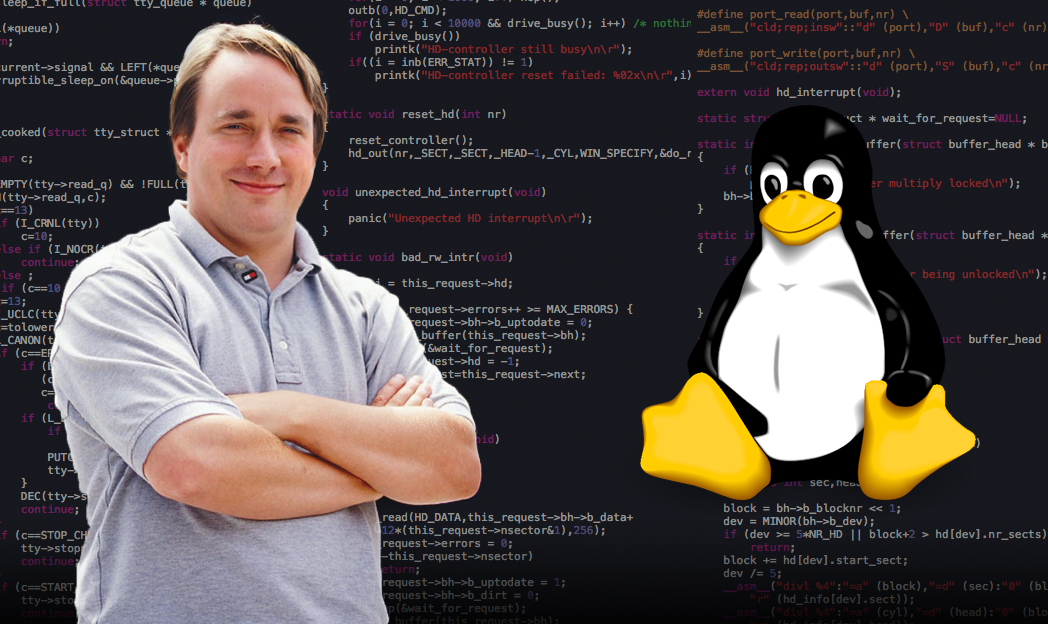
\includegraphics[height=4cm, width=6cm]{linus-torvalds-interviu.png}
\end{block}
\end{frame}
%\break
\begin{frame}{Différenciations}
    \begin{block}
        \raggedright Les parties GNU et Linux d’un système d’exploitation GNU/LINUX sont indépendantes, on trouve aussi bien des systèmes avec Linux sans la partie GNU tels qu'Android, ou des systèmes GNU sans Linux telque GNU/Hurd.
    \end{block}
\end{frame}

\section{Principe}
\begin{frame}{Principe}
\begin{block}
  \raggedright    
  \raggedright Les différentes distributions changent entièrement l'aspect et la fonction de Linux. Elles s'étendent du système complet (développé par des entreprises), pour des ordinateurs personnels ou des serveurs, à des systèmes légers (souvent développés par des volontaires) qui s'installent sur une clé mémoire USB ou sur de vieux ordinateurs.
\end{block}
\end{frame}
%\titlespacing{#1}{#2}{#3}
%\subsection{First Subsection}

%\begin{frame}{First Slide Title}{Optional Subtitle}
 % \begin{itemize}
  %\item {
   % My first point.
  %}
  %\item {
   % My second point.
  %}
  %\end{itemize}
%\end{frame}

%\subsection{Second Subsection}

% You can reveal the parts of a slide one at a time
% with the \pause command:
%\begin{frame}{Second Slide Title}
  %\begin{itemize}
  %\item {
   % First item.
    %\pause % The slide will pause after showing the first item
  %}
  %\item {   
  %  Second item.
  %}
  % You can also specify when the content should appear
  % by using <n->:
  %\item<3-> {
    %Third item.
  %}
  %\item<4-> {
   % Fourth item.
  %}
  % or you can use the \uncover command to reveal general
  % content (not just \items):
  %\item<5-> {
   % Fifth item. \uncover<6->{Extra text in the fifth item.}
  %}
  %\end{itemize}
%\end{frame}

%\section{}

\raggedright 
\begin{frame}

\begin{block}{Architecture Logicielle d'une distribution}
\begin{itemize}
    \item Exploitation du concept de couche d'abstraction matérielle
\end{itemize}

\centering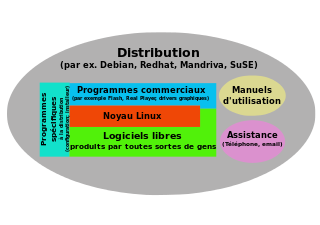
\includegraphics[height=5cm, width=8cm]{d.png}
\end{block}
\end{frame}

%\section{Noyau Linux}
\section{Différence entre distribution commerciales et non commerciales}
\begin{frame}
\begin{block}{Commerciales}
\begin{itemize}[<+-| alert@+>]
\item Distribution à but lucratif (developpée par une entreprise) 
\item Choisie et assemble les logiciels qui composent la distribution.\\ 
\item Proposent généralement des versions gratuites.\\
\item Exemple: Ubuntu, RedHat, Mandriva...
\end{itemize}
\end{block}
\begin{block}{Non Commerciales}
\begin{itemize}[<+-| alert@+>]
\item Distribution à but non lucratif (developée par une communauté) 
\item Proposent des versions non gratuites
\item aucun service d'assistence n'est fournis
\item Exemple: Debian, ArchLinux...
\end{itemize}
\end{block}
\end{frame}

\section{Principales Distributions}
\subsection{Distribution Grand Public }
\begin{frame}
%\renewcommand{\arraystretch}{1}
%{\renewcommand{\arraystretch}{0:1} %donne la distance entre les lignes%
%{\setlength{\tabcolsep}{0.12cm} %donne la distance entre les collones%
\begin{tabular}{|c|p{8cm}|p{8cm}|p{8cm}|p{8cm}|}
\hline

\includegraphics[width=1cm]{f.png} & Fedora est une distribution communautaire supervisée par Red Hat, basée sur le système de gestion de paquetages logiciels RPM.\\
\hline

\includegraphics[width=1cm]{l.png} & Trisquel est un système d’exploitation fondé sur GNU/Linux.\\
  \hline
  
\includegraphics[width=1cm]{m.png} &  Manjaro  est une distribution basée sur Arch Linux.\\
  \hline
   \centering
\includegraphics[width=1cm]{u.png} & \href{https://fr.wikipedia.org/wiki/Ubuntu}{Ubuntu} est basé sur Debian.C'est une distribution commerciale orientée vers le grand public distribuée par Canonical.\\
   \hline
\end{tabular}
\end{frame}
\subsection{Système P\`ere}
\begin{frame}
\begin{tabular}{|c|p{8cm}|p{8cm}|p{8cm}|p{8cm}|}
\hline

\includegraphics[width=1cm]{red.png} & Red Hat (officiellement Red Hat Enterprise Linux ou RHEL) est une distribution commerciale largement répandue dans les entreprises (surtout aux États-Unis).\\
\hline

\includegraphics[width=1cm]{deb.png} & Debian est une distribution non commerciale régie par le contrat social Debian. \\
\hline

\includegraphics[width=1cm]{sack.jpg} & Slackware est l'une des plus anciennes distributions existantes.\\
\hline

\includegraphics[width=1cm]{gen.png} & Gentoo est une distribution caractérisée par sa gestion des paquetages.\\
\hline
\end{tabular}
\end{frame}

\section{Critère de distinction des distribution}
%\subsection{Architecture matérielle supportée}
\begin{frame}
\begin{itemize}[<+-| alert@+>]
    \item Architecture matérielle supportée
    \item Gestionnaire de paquet
    \begin{itemize}[<+-| alert@+>]
    \item distribution de paquet binaire
    \item distribution basée sur la compilation
    \end{itemize}
    \item Formats des paquetages 
    \item Stabilité
    \item Puissance de la machine
    
\end{itemize}
\end{frame}
\begin{frame}
    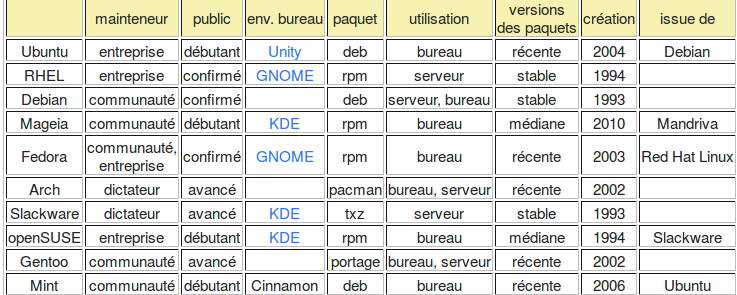
\includegraphics[width=10cm]{capt.png}
    \end{frame}
\section{Exemple d'installation d'une distribution}
\begin{frame}
    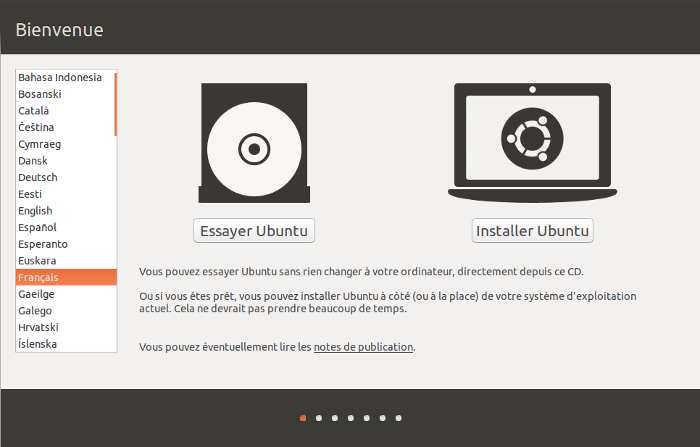
\includegraphics[width=10cm]{ubun.jpeg}
    \end{frame}
    \begin{frame}
     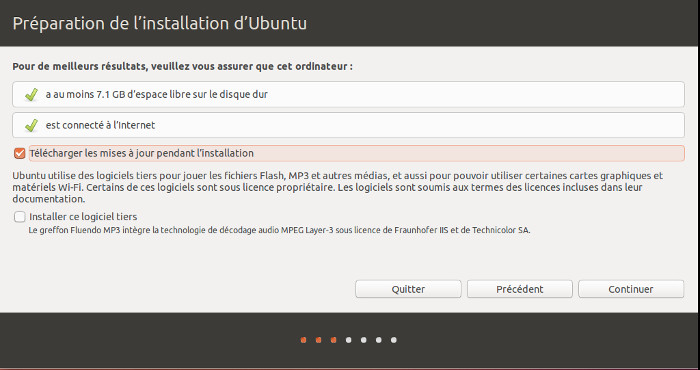
\includegraphics[width=10cm]{Ubuntu.jpeg}
\end{frame}
\begin{frame}
    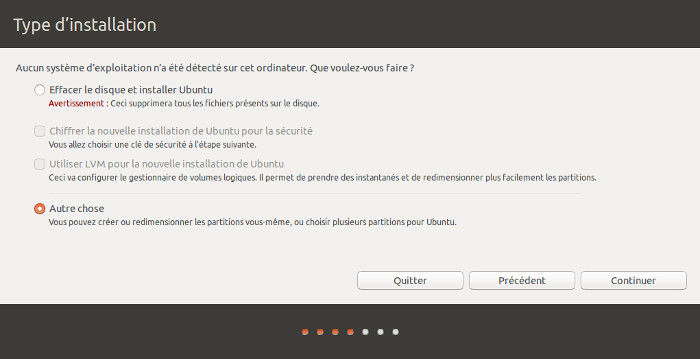
\includegraphics[width=10cm]{partit.jpeg}
    \end{frame}
    \begin{frame}
    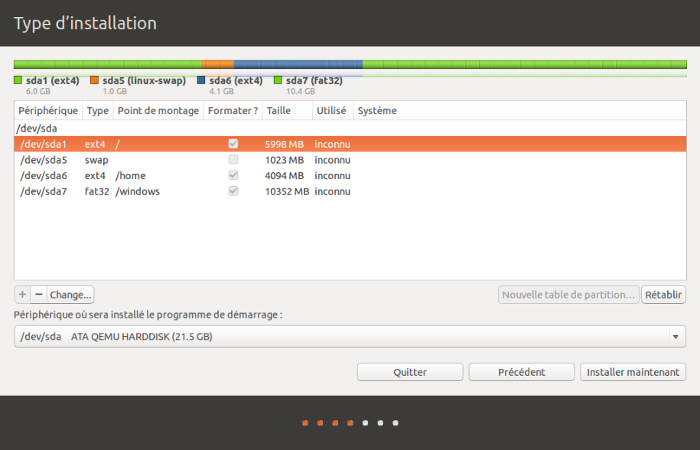
\includegraphics[width=10cm]{part.jpeg}
    \end{frame}
    \begin{frame}
    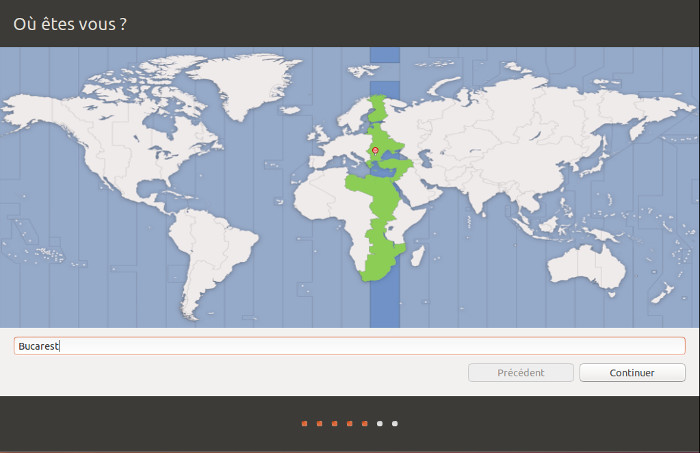
\includegraphics[width=10cm]{heur.jpeg}
    \end{frame}
    \begin{frame}
    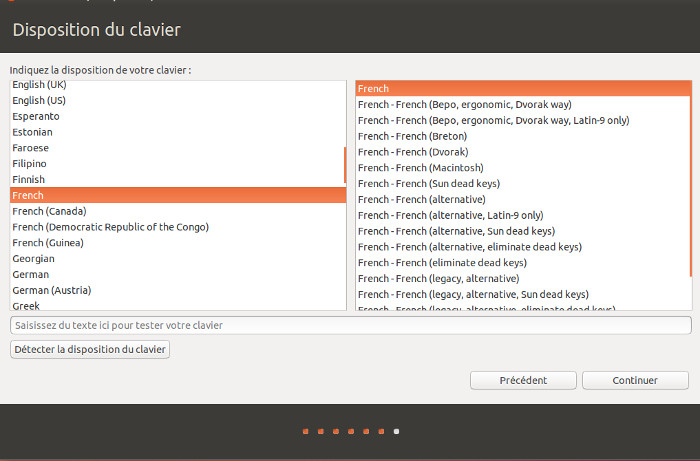
\includegraphics[width=10cm]{dispo.jpeg}
    \end{frame}
    \begin{frame}
    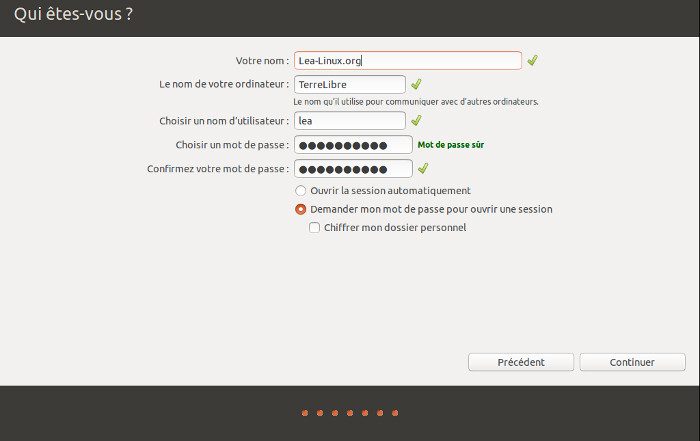
\includegraphics[width=10cm]{qui.jpeg}
    \end{frame}
    \begin{frame}
    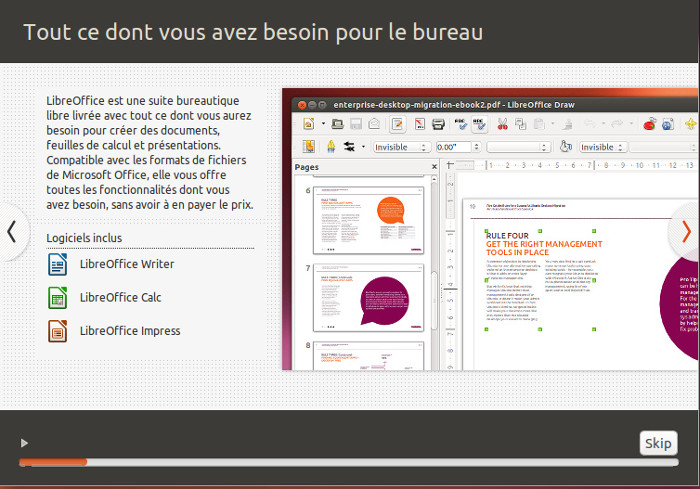
\includegraphics[width=10cm]{bur.jpeg}
    \end{frame}
    \begin{frame}
    
\includegraphics[width=10cm]{ins.jpeg}
    \end{frame}
\section{Conclusion}
\begin{frame}
\begin{block}{Que choisir?}
    Ayant utilisé Ubuntu tous les deux, on a été conquis par sa simplicité d'utilisation. Je vous conseille de baser vos choix sur les critères suivants:
    \begin{itemize}
        \item est-ce que la complexité de l'installation et de la configuration est à mon niveau ? 
        \item est-ce que l'essai de la version Live m'a plu ? 
        \item est-ce que la communauté autour est importante ? 
    \end{itemize}
    Au final, comme toujours, toutes se valent plus ou moins, tout dépend de ce que vous en attendez... 
\end{block}    
\end{frame}



%\subsection{Another Subsection}

\end{document}


